%%%%%%%%%%%%%%%%%%%%%%%%%%%%%%%%%%%%%%%%%%%%%%%%%%%%%%%
\documentclass{article}
%%%%%%%%%%%%%%%%%%%%%%%%%%%%%%%%%%%%%%%%%%%%%%%%%%%%%%%
\usepackage[utf8]{vietnam}
%%%%%%%%%%%%%%%%%%%%%%%%%%%%%%%%%%%%%%%%%%%%%%%%%%%%%%%
\usepackage{graphicx}
%%%%%%%%%%%%%%%%%%%%%%%%%%%%%%%%%%%%%%%%%%%%%%%%%%%%%%%
\usepackage{hyperref}
%%%%%%%%%%%%%%%%%%%%%%%%%%%%%%%%%%%%%%%%%%%%%%%%%%%%%%%
\usepackage{xcolor}
\pagecolor[RGB]{40, 42, 54} % Đặt màu nền
\color[RGB]{18, 161, 24} % Đặt màu chữ
%%%%%%%%%%%%%%%%%%%%%%%%%%%%%%%%%%%%%%%%%%%%%%%%%%%%%%%
\usepackage{float} % Cố định hình ảnh [H]
%%%%%%%%%%%%%%%%%%%%%%%%%%%%%%%%%%%%%%%%%%%%%%%%%%%%%%%
\begin{document}
%%%%%%%%%%%%%%%%%%%%%%%%%%%%%%%%%%%%%%%%%%%%%%%%%%%%%%%
\tableofcontents
\newpage
%%%%%%%%%%%%%%%%%%%%%%%%%%%%%%%%%%%%%%%%%%%%%%%%%%%%%%%
\listoffigures
\newpage
%%%%%%%%%%%%%%%%%%%%%%%%%%%%%%%%%%%%%%%%%%%%%%%%%%%%%%%
\section{Tuần 3: Xây dựng dashboard}
%%%%%%%%%%%%%%%%%%%%%%%%%%%%%%%%%%%%%%%%%%%%%%%%%%%%%%%
\subsection{Bài 1}

\begin{figure}[H]
\centering
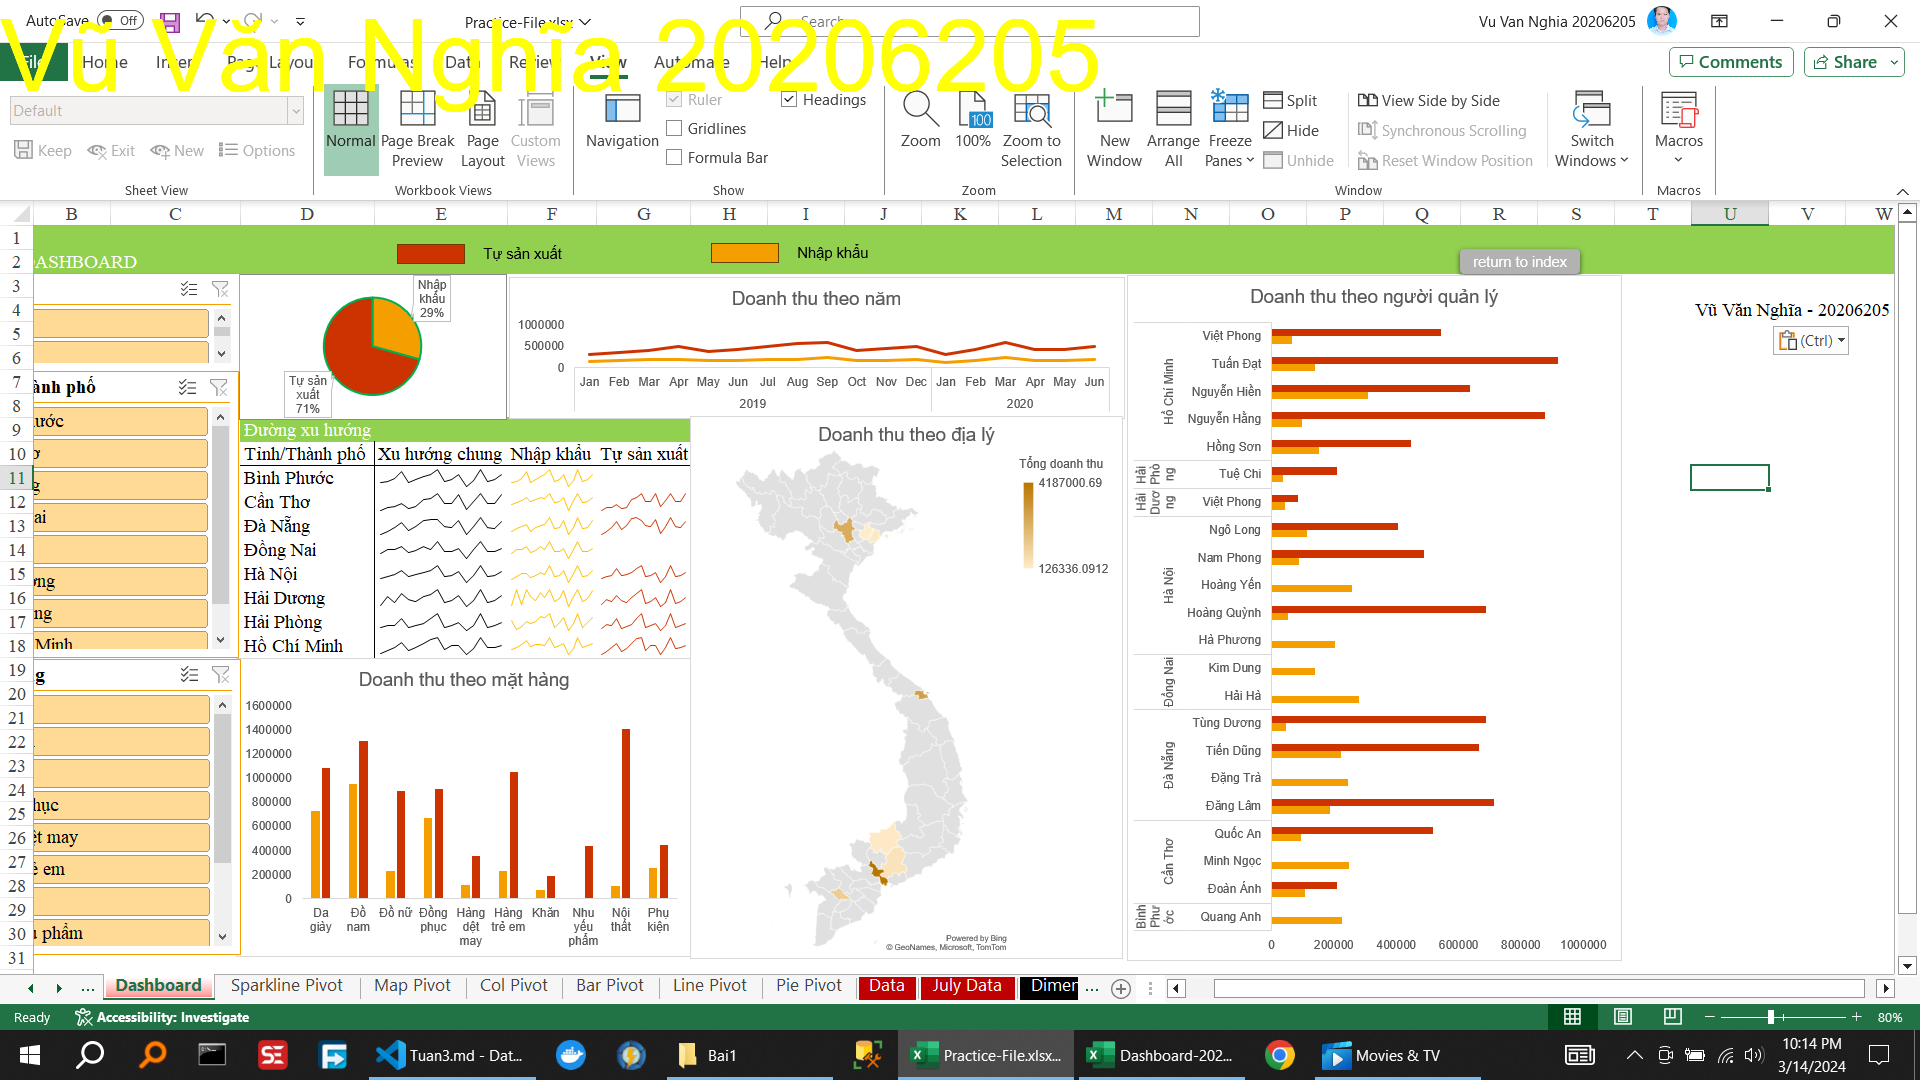
\includegraphics[scale = 0.15]{Bai1/ThucHanh/0.png}
\caption{Thực hành tạo Dashboard theo video}
\end{figure}

% <!-- \caption{Thực hành phân tích Dashboard} -->

% <!-- B1. Đọc dashboard, phân tích -->

% Dashboard dùng để

% Dashboard có các biểu đồ:
% ...

% <!-- B2. Xác định các chiều (DIM), các các yếu tố phân tích (FACT) -->

\begin{figure}[H]
\centering
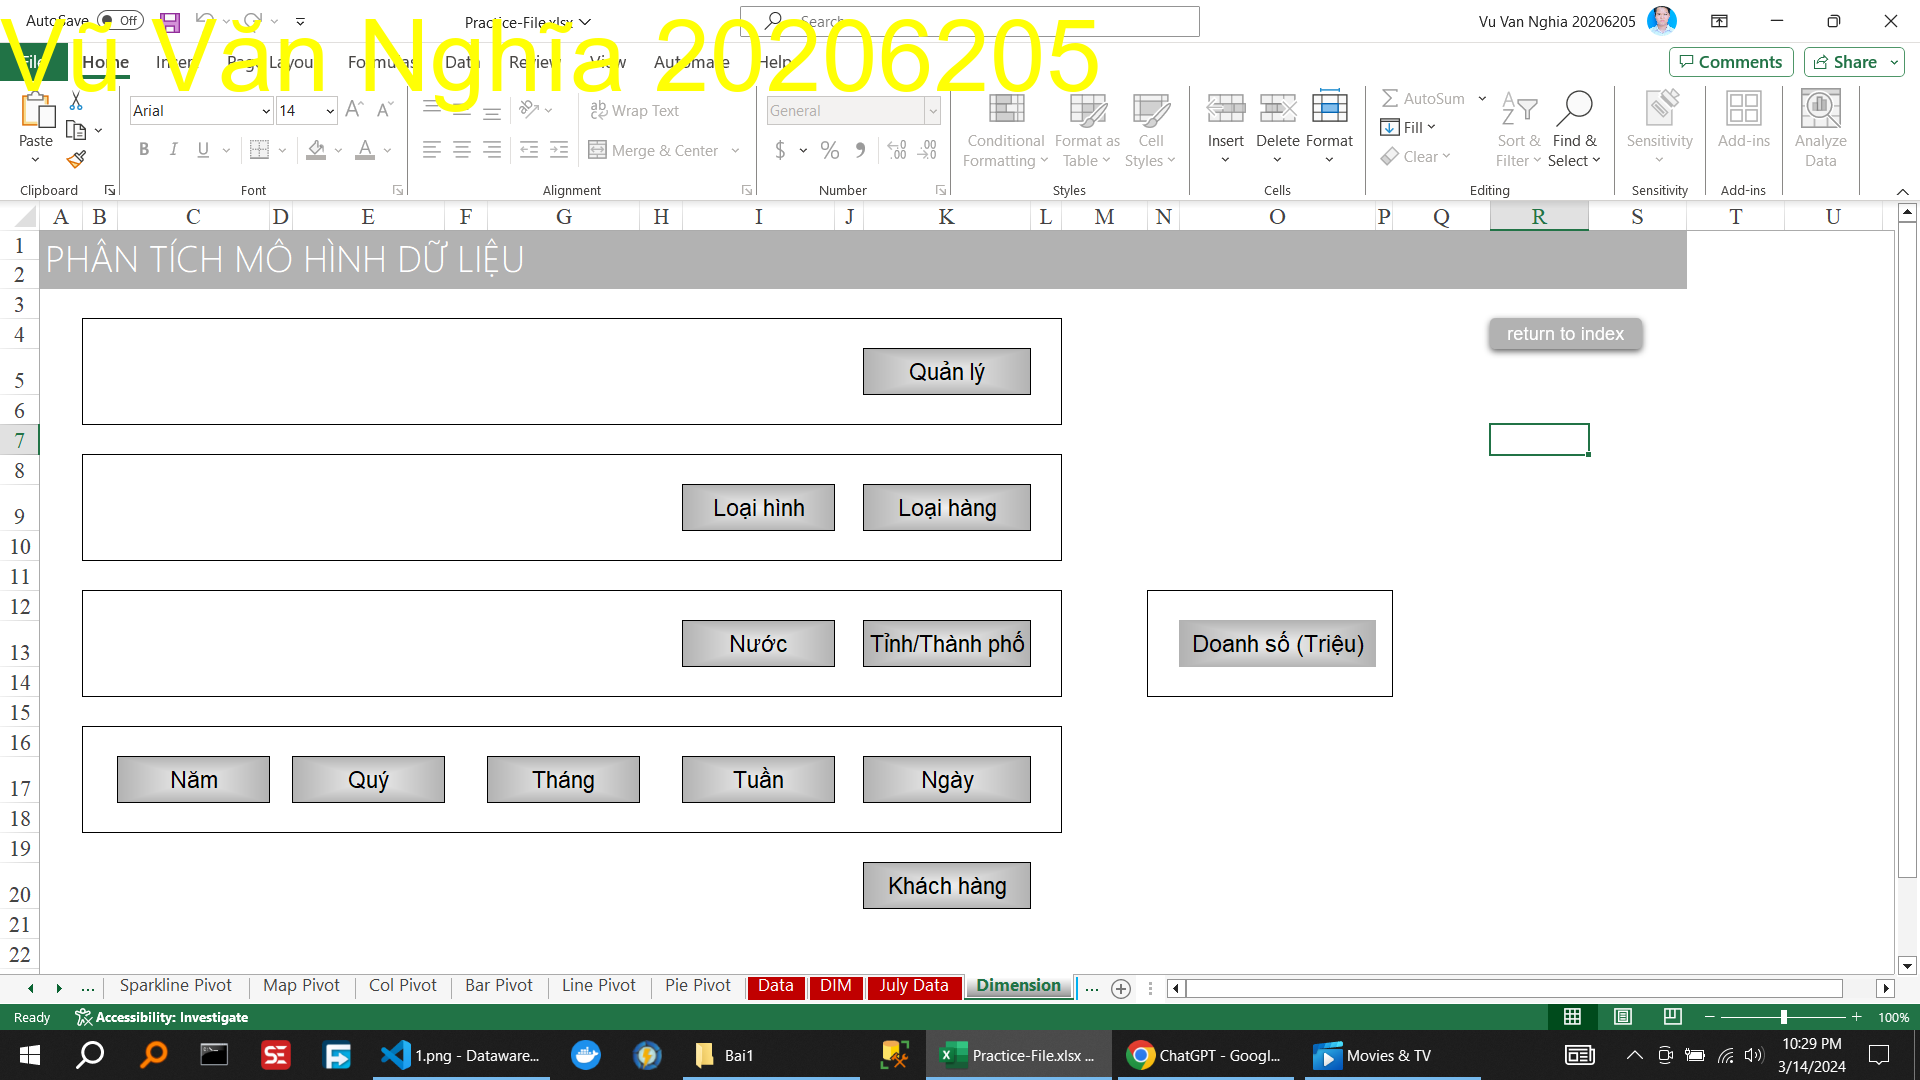
\includegraphics[scale = 0.15]{Bai1/ThucHanh/1.png}
% \caption{Thực hành tạo Dashboard theo video}
\end{figure}

% ảnh ...
% text...

% Bước 2: Xác định Các Chiều (DIM) và Các Yếu Tố Phân Tích (FACT)
% Xác định các chiều (DIM) là các khía cạnh của dữ liệu bạn muốn phân tích. Ví dụ: Thời gian, Năm, Loại hình Sản xuất, Tỉnh/Thành phố, Nước, Quản lý, Mặt hàng, Khách hàng.
% Xác định các yếu tố phân tích (FACT) là các dữ liệu số hoặc thông tin mà bạn muốn phân tích. Ví dụ: Doanh số (Triệu).

% <!-- B3. Sử dụng công cụ Remove Duplicate để tạo ra con voi khái niệm các chiều. -->

\begin{figure}[H]
\centering
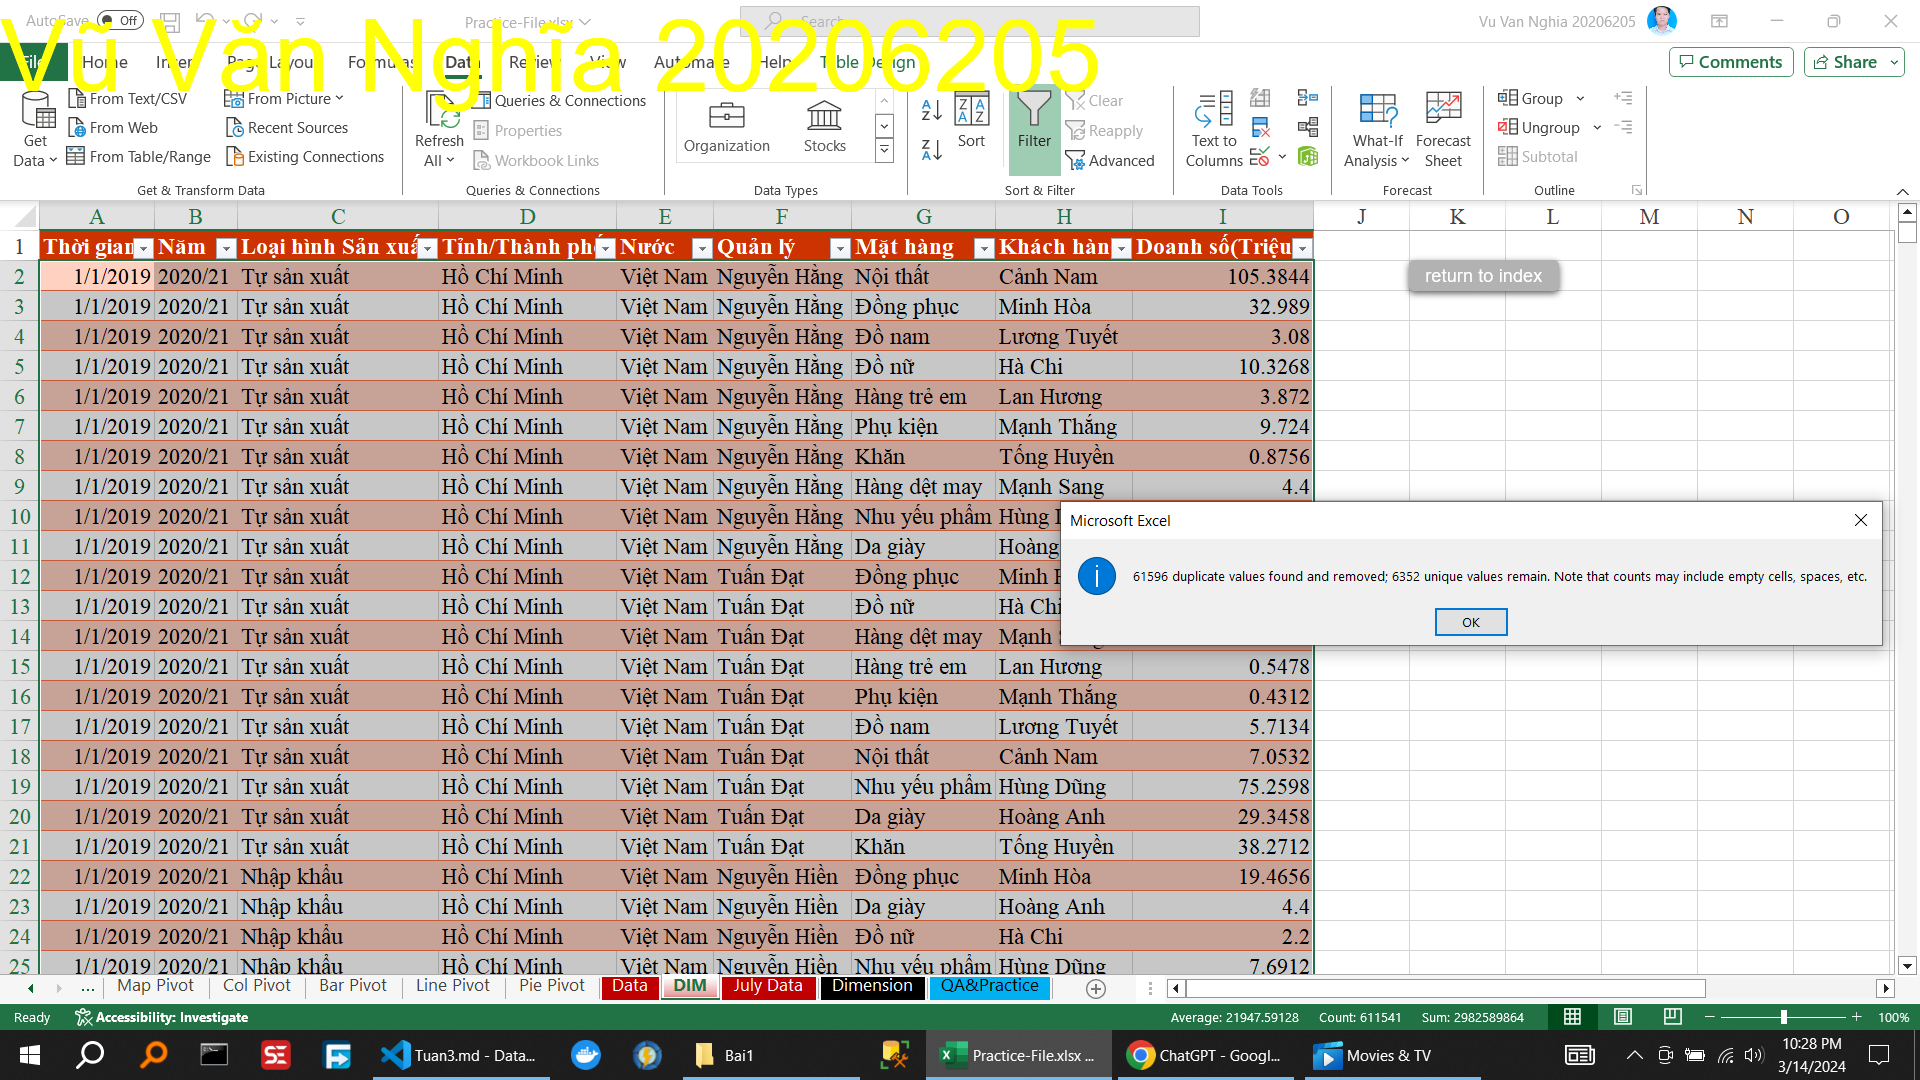
\includegraphics[scale = 0.15]{Bai1/ThucHanh/2.png}
% \caption{Thực hành tạo Dashboard theo video}
\end{figure}
%%%%%%%%%%%%%%%%%%%%%%%%%%%%%%%%%%%%%%%%%%%%%%%%%%%%%%%
\subsection{Bài 2}

% \begin{figure}[H]
% \centering
% 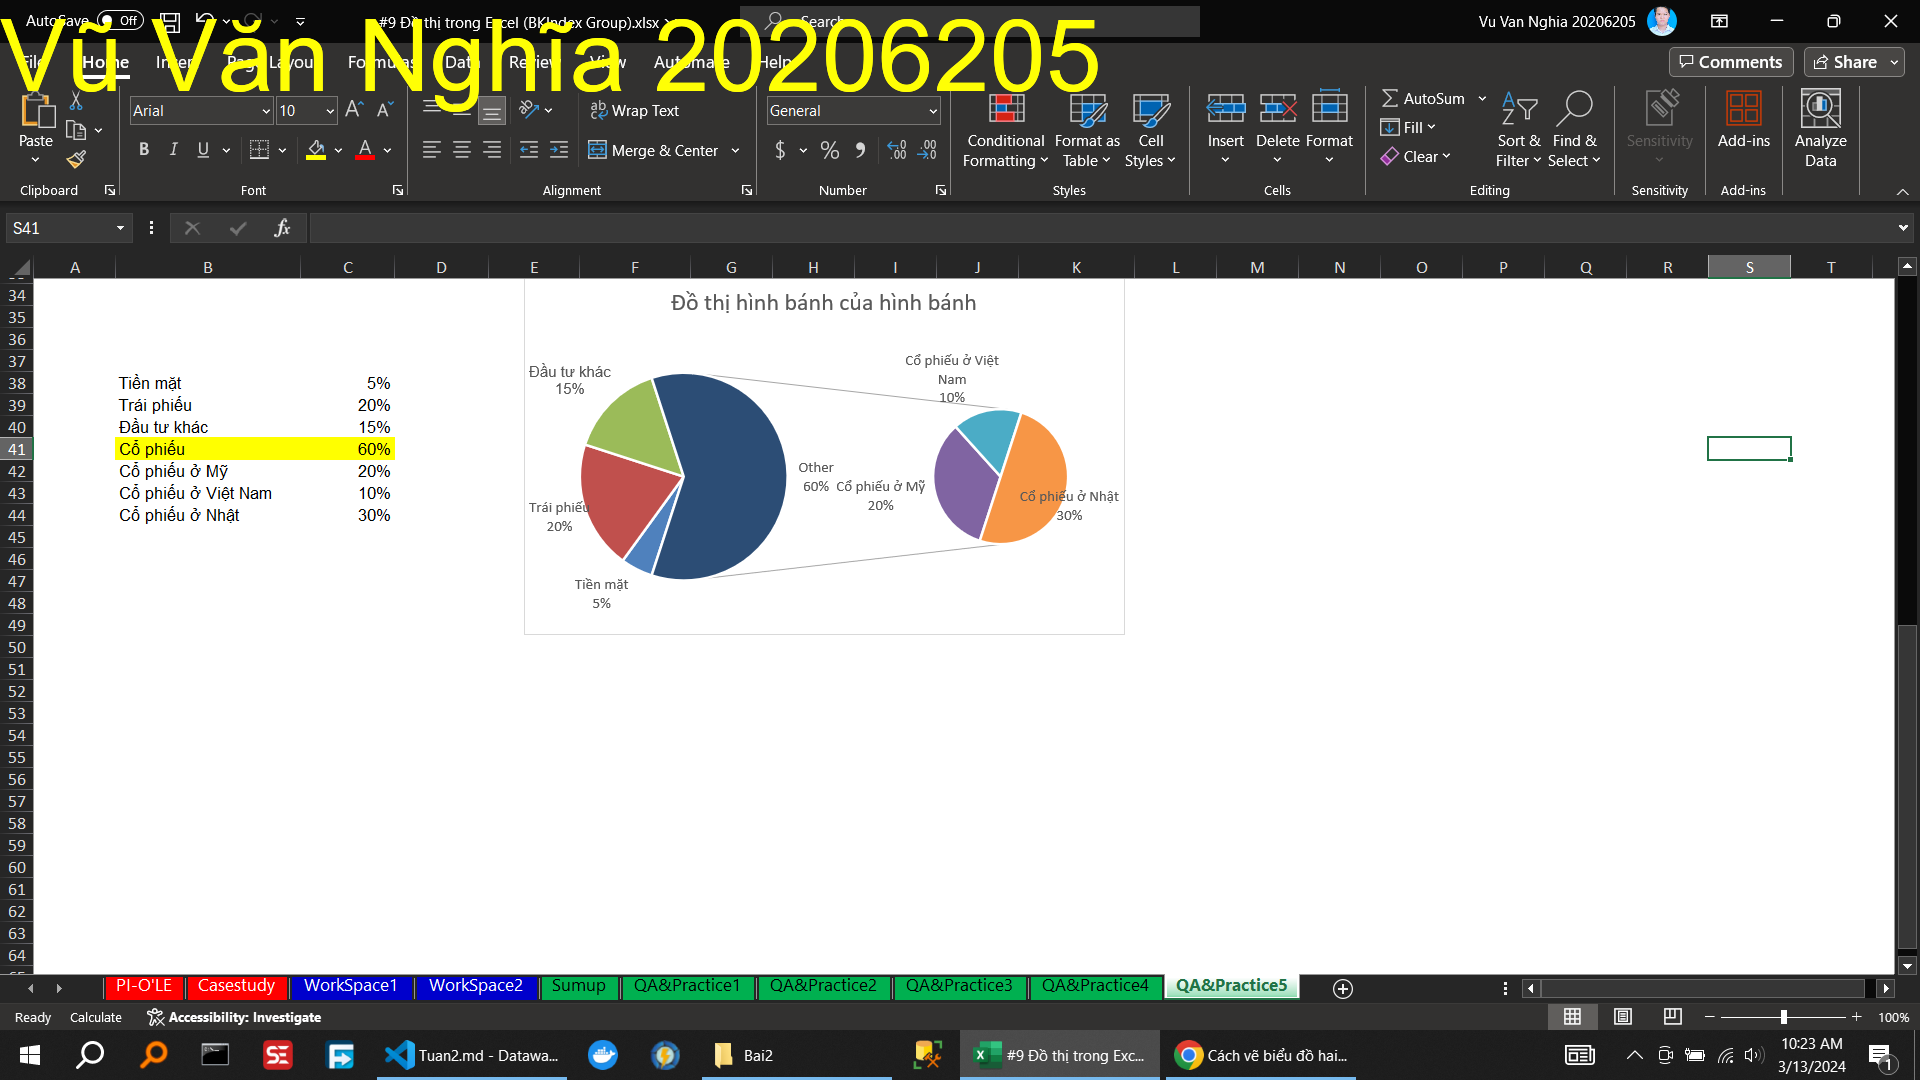
\includegraphics[scale = 0.15]{Bai2/ThucHanh/3.png}
% \caption{Thực hành vẽ đồ thị hình bánh của hình bánh}
% \end{figure}

%%%%%%%%%%%%%%%%%%%%%%%%%%%%%%%%%%%%%%%%%%%%%%%%%%%%%%%
\end{document}
%%%%%%%%%%%%%%%%%%%%%%%%%%%%%%%%%%%%%%%%%%%%%%%%%%%%%%%